\section{Sektionsführung / Platoon Lead (PLT)}
\begin{wrapfigure}{r}{0.5\textwidth}
	\centering 
	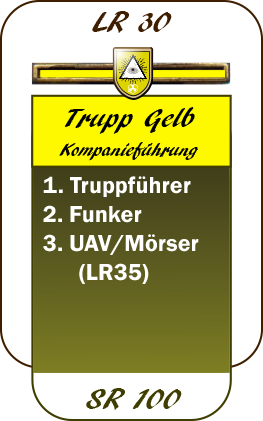
\includegraphics[width=0.35\textwidth]{./img/truppenordnung/sektionsfuehrung/sektionsfuehrung.png}
	\caption{Beispiel einer Sektionsführung}
\end{wrapfigure}	

Die Sektionsführung ist ein Bindeglied zwischen OPL und Zugführung, um die OPL zu entlasten. Einer Sektionsführung sind mindestens zwei, maximal vier Züge unterstellt. Ab drei Zügen in einer Mission ist die Sektionsführung zwingend erforderlich, darunter optional.\\
Die Sektionsführung ist folgendermaßen aufgebaut:
\begin{itemize}
	\item Sektionsführer / Platoon Lead (PLT): Er leitet die ihm untergeordneten Züge. Kommuniziert wird über Long-Range - entweder über die individuellen Frequenzen der einzelnen Züge oder über die Task-Force-Frequenz (siehe nächstes Kapitel).
	\item Funker / Radio Operator (RO): Übernimmt die Kommunikation zur OPL und anderen Einheiten.
\end{itemize}
Ergänzt werden kann die Sektionsführung bei Bedarf durch einen Gefechtssanitäter / Combat Medic (CM) zur Versorgung im Feld.
